\secrel{Задание на исследование выключателя}

Найдите маленький переключатель, аккуратно разберите его, нарисуйте конструкцию,
и объясните как он работает. Убедитесь, что вы поняли цель пружин(ы).
Вот упрощенные рисунки небольшого переключателя, когда он находится в разных
позициях. Когда переключатель включен, электричество может течь, когда он
разомкнут, цепь разорвана.

\noindent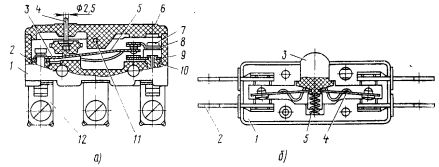
\includegraphics[width=0.95\textwidth]{bcollis/switch.jpg}
